
%{{第七回}}{第七回}}

\chapter{送宫花周瑞叹英莲\\谈肄业秦钟结宝玉}\label{part0011_split_000.htmlux5cux23calibre_pb_0}

{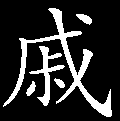
\includegraphics[width=3mm]{../Images/00005}苦尽甘来递转,正强忽弱谁明?惺惺自古惜惺惺,世运文章操劲。无缝机关难见,多才笔墨偏精。有情情处特无情,何是人人不醒?}

题曰:

十二花容色最新,不知谁是惜花人?

相逢若问名何氏?家住江南姓本秦。

话说周瑞家的送了刘姥姥去后,便上来回王夫人话。{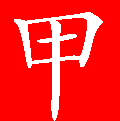
\includegraphics[width=3mm]{../Images/00002}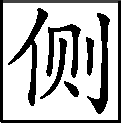
\includegraphics[width=3mm]{../Images/00011}\footnotesize \kaishu 不回凤姐,却回王夫人,不交代处,正交代得清楚。}谁知王夫人不在上房,问丫鬟们时,方知往薛姨妈那边闲话去了。{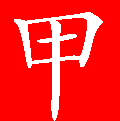
\includegraphics[width=3mm]{../Images/00002}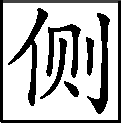
\includegraphics[width=3mm]{../Images/00011}\footnotesize \kaishu 文章只是随笔写来,便有流离生动之妙。}周瑞家的听说,便转东角门出至东院,往梨香院来。刚至院门前,只见王夫人的丫鬟名金钏儿{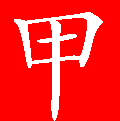
\includegraphics[width=3mm]{../Images/00002}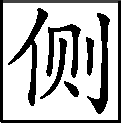
\includegraphics[width=3mm]{../Images/00011}\footnotesize \kaishu 金钏、宝钗互相映射。妙!}者,和一个才留了头的小女孩儿{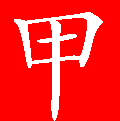
\includegraphics[width=3mm]{../Images/00002}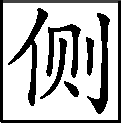
\includegraphics[width=3mm]{../Images/00011}\footnotesize \kaishu 莲卿别来无恙否?}站立台矶上顽。见周瑞家的来了,便知有话回,因向内努嘴儿。{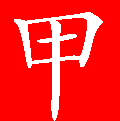
\includegraphics[width=3mm]{../Images/00002}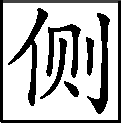
\includegraphics[width=3mm]{../Images/00011}\footnotesize \kaishu 画。}周瑞家的轻轻掀帘进去,只见王夫人和薛姨妈长篇大套的说些家务人情等语。{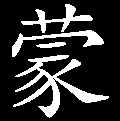
\includegraphics[width=3mm]{../Images/00006}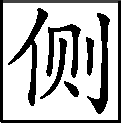
\includegraphics[width=3mm]{../Images/00011}\footnotesize \kaishu 非此等事,不能长篇大套。}

周瑞家的不敢惊动,遂进里间来。{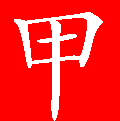
\includegraphics[width=3mm]{../Images/00002}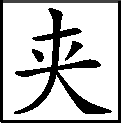
\includegraphics[width=3mm]{../Images/00012}\footnotesize \kaishu 总用双歧岔路之笔,令人估料不到之文。}只见薛宝钗{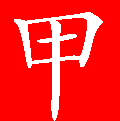
\includegraphics[width=3mm]{../Images/00002}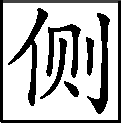
\includegraphics[width=3mm]{../Images/00011}\footnotesize \kaishu 自入梨香院,至此方写。}穿着家常衣服,{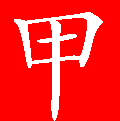
\includegraphics[width=3mm]{../Images/00002}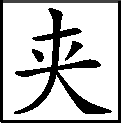
\includegraphics[width=3mm]{../Images/00012}\footnotesize \kaishu 好!写一人换一副笔墨,另出一花样。 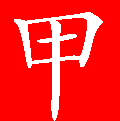
\includegraphics[width=3mm]{../Images/00002}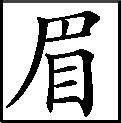
\includegraphics[width=3mm]{../Images/00010}\footnotesize \kaishu ``家常爱着旧衣裳''是也。}头上只散挽着?儿,坐在炕里边,伏在小炕几上,同丫鬟莺儿正描花样子呢。{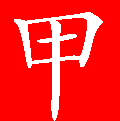
\includegraphics[width=3mm]{../Images/00002}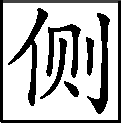
\includegraphics[width=3mm]{../Images/00011}\footnotesize \kaishu 一幅《绣窗仕女图》,亏想得周到。}见他进来,宝钗便放下笔,转过身来,满面堆笑让:``周姐姐坐。''周瑞家的也忙陪笑问:``姑娘好?''一面炕沿边坐了,因说:``这有两三天也没见姑娘到那边逛逛去,只怕是你宝玉兄弟冲撞了你不成?''{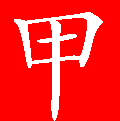
\includegraphics[width=3mm]{../Images/00002}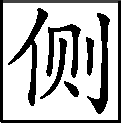
\includegraphics[width=3mm]{../Images/00011}\footnotesize \kaishu 一人不漏,一笔不板。}宝钗笑道:``那里的话。只因我那种病又发了两天,{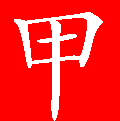
\includegraphics[width=3mm]{../Images/00002}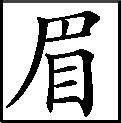
\includegraphics[width=3mm]{../Images/00010}\footnotesize \kaishu ``那种病''。``那''字与前二玉``不知因何''二``又''字,皆得天成地设之体;且省却多少闲文,所谓``惜墨如金''是也。}所以且静养两日。''{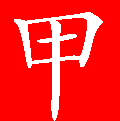
\includegraphics[width=3mm]{../Images/00002}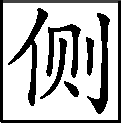
\includegraphics[width=3mm]{../Images/00011}\footnotesize \kaishu 得空便入。}周瑞家的道:``正是呢,姑娘到底有什么病根儿,也该趁早儿请了大夫来,好生开个方子,认真吃几剂药,一势除了根才好。小小的年纪倒坐下个病根,也不是顽的。''宝钗听说,便笑道:``再不要提吃药,为这病请大夫、吃药,也不知白花了多少银子钱呢。凭你什么名医仙药,总不见一点儿效。后来还亏了一个秃头和尚,{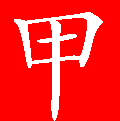
\includegraphics[width=3mm]{../Images/00002}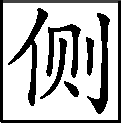
\includegraphics[width=3mm]{../Images/00011}\footnotesize \kaishu 奇奇怪怪,真如云龙作雨,忽隐忽现,使人逆料不到。}说专治无名之症,因请他看了。他说我这是从胎里带来的一股热毒,{{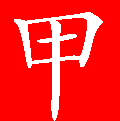
\includegraphics[width=3mm]{../Images/00002}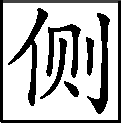
\includegraphics[width=3mm]{../Images/00011}\footnotesize \kaishu 凡心偶炽,是以孽火齐攻。 }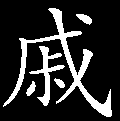
\includegraphics[width=3mm]{../Images/00005}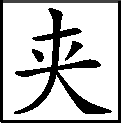
\includegraphics[width=3mm]{../Images/00012}\footnotesize \kaishu ``热毒''二字画出富家夫妇,图一时遗害于子女,而可不谨慎!}幸而我先天结壮,还不相干。{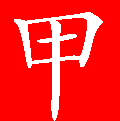
\includegraphics[width=3mm]{../Images/00002}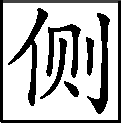
\includegraphics[width=3mm]{../Images/00011}\footnotesize \kaishu 浑厚故也,假使颦、凤辈,不知又何如治之。}若吃凡药,是不中用的。他就说了一个海上方,又给了一包末药作引,异香异气的。不知是那里弄来的。他说发了时吃一丸就好。倒也奇怪,这倒效验些。''{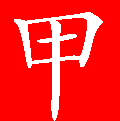
\includegraphics[width=3mm]{../Images/00002}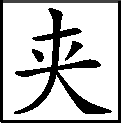
\includegraphics[width=3mm]{../Images/00012}\footnotesize \kaishu 卿不知从那里弄来,余则深知。是从放春山采来,以灌愁海水和成,烦广寒玉兔捣碎,在太虚幻境空灵殿上炮制配合者也。}

周瑞家的因问道:``不知是个什么海上方儿?姑娘说了,我们也记着,说与人知道,倘遇见这样的病,也是行好的事。''宝钗见问,乃笑道:``不问这方儿还好,若问起这方儿,真真把人琐碎坏了。东西药料一概都有,现易得的,只难得`可巧'二字:要春天开的白牡丹花蕊十二两,{{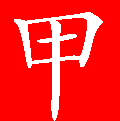
\includegraphics[width=3mm]{../Images/00002}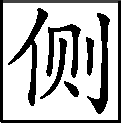
\includegraphics[width=3mm]{../Images/00011}\footnotesize \kaishu 凡用``十二''字样,皆照应十二钗。 }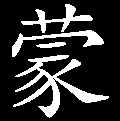
\includegraphics[width=3mm]{../Images/00006}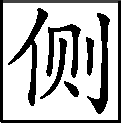
\includegraphics[width=3mm]{../Images/00011}\footnotesize \kaishu 周岁十二月之象。}夏天开的白荷花蕊十二两,秋天开的白芙蓉花蕊十二两,冬天开的白梅花蕊十二两。将这四样花蕊,于次年春分这日晒干,和在末药一处,一齐研好。又要雨水这日的雨水十二钱,\ldots{}\ldots{}''周瑞家的忙道:``嗳哟!这样说来,这就得一二年的工夫。倘或雨水这日不下雨水,又怎处呢?''宝钗笑道:``所以了,那里有这样可巧的雨,便没雨也只好再等罢了。白露这日的露水十二钱,霜降这日的霜十二钱,小雪这日的雪十二钱。把这四样水调匀,和了丸药,再加蜂蜜十二钱,白糖十二钱,丸了龙眼大的丸子,盛在旧磁罐内,埋在花根底下。若发了病时,拿出来吃一丸,用十二分黄柏{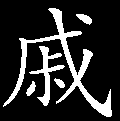
\includegraphics[width=3mm]{../Images/00005}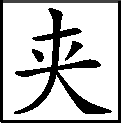
\includegraphics[width=3mm]{../Images/00012}\footnotesize \kaishu 历着炎凉,知着甘苦,虽离别亦自能安,故名曰冷香丸。又以谓香可冷得,天下一切无不可冷者。}煎汤送下。''{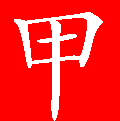
\includegraphics[width=3mm]{../Images/00002}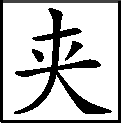
\includegraphics[width=3mm]{../Images/00012}\footnotesize \kaishu 末用黄柏更妙。可知``甘苦''二字,不独十二钗,世皆同有者。}

周瑞家的听了,笑道:``阿弥陀佛,真坑死了人!\href{../Text/part0011_split_000.html\#lnkback_1_a}{\textsuperscript{①}}等十年未必都这样巧呢。''宝钗道:``竟好,自他说了去后,一二年间可巧都得了,好容易配成一料。如今从南带至北,现就埋在梨花树下。''{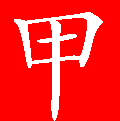
\includegraphics[width=3mm]{../Images/00002}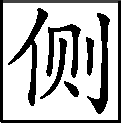
\includegraphics[width=3mm]{../Images/00011}\footnotesize \kaishu ``梨香''二字有着落,并未白白虚设。}周瑞家的又道:``这药可有名字没有呢?''宝钗道:``有。{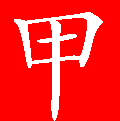
\includegraphics[width=3mm]{../Images/00002}\includegraphics[width=3mm]{../Images/00011}\footnotesize \kaishu 一字句。}这也是癞和尚说下的,叫作`冷香丸'。''{\includegraphics[width=3mm]{../Images/00002}\includegraphics[width=3mm]{../Images/00011}\footnotesize \kaishu 新雅,奇甚。}周瑞家的听了点头儿,因又说:``这病发了时到底觉怎样?''宝钗道:``也不觉什么,只不过喘嗽些,吃一丸也就罢了。''{\includegraphics[width=3mm]{../Images/00002}\includegraphics[width=3mm]{../Images/00012}\footnotesize \kaishu 以花为药,可是吃烟火人想得出者?诸公且不必问其事之有无,只据此新奇妙文悦我等心目,便当浮一大白。}

周瑞家的还欲说话时,忽听王夫人问:{\includegraphics[width=3mm]{../Images/00006}\includegraphics[width=3mm]{../Images/00011}\footnotesize \kaishu 了结得齐整。}``是谁在里头?''周瑞家的忙出去答应了,趁便回了刘姥姥之事。略待半刻,见王夫人无话,方欲退出,{\includegraphics[width=3mm]{../Images/00002}\includegraphics[width=3mm]{../Images/00012}\footnotesize \kaishu 行文原只在一二字,便有许多省力处。不得此窍者,便在窗下百般扭捏。}薛姨妈忽又笑道:{\includegraphics[width=3mm]{../Images/00002}\includegraphics[width=3mm]{../Images/00012}\footnotesize \kaishu ``忽''字``又''字与``方欲''二字对射。}``你且站住。我有一宗东西,你带了去罢。''说着便叫香菱。{\includegraphics[width=3mm]{../Images/00002}\includegraphics[width=3mm]{../Images/00012}\footnotesize \kaishu 二字仍从``莲''上起来。盖``英莲''者,``应怜''也,``香菱''者亦``相怜''之意。此是改名之``英莲''也。}帘栊响处,方才和金钏儿顽的那个小女孩子进来了,问:``奶奶叫我作什么?''{\includegraphics[width=3mm]{../Images/00002}\includegraphics[width=3mm]{../Images/00012}\footnotesize \kaishu 这是英莲天生成的口气,妙甚!}薛姨妈道:``把那匣子里的花儿拿来。''香菱答应了,向那边捧了个小锦匣来。薛姨妈乃道:``这是宫里头作的新鲜样法堆纱花十二枝。昨儿我想起来,白放着可惜旧了,何不给他们姊妹们戴去。昨儿要送去,偏又忘了。你今儿来的巧,就带了去罢。你家的三位姑娘,每人两枝,下剩六枝,送林姑娘两枝,那四枝给了凤哥儿罢。''{\includegraphics[width=3mm]{../Images/00002}\includegraphics[width=3mm]{../Images/00011}\footnotesize \kaishu 妙文!今古小说中可有如此口吻者?}王夫人道:``留着给宝丫头戴罢了,又想着他们。''薛姨妈道:``姨妈不知道,宝丫头古怪{\includegraphics[width=3mm]{../Images/00002}\includegraphics[width=3mm]{../Images/00011}\footnotesize \kaishu ``古怪''二字,正是宝卿身份。}呢,他从来不爱这些花儿粉儿的。''{\includegraphics[width=3mm]{../Images/00002}\includegraphics[width=3mm]{../Images/00012}\footnotesize \kaishu 可知周瑞一回,正为宝、菱二人所有,正《石头记》得力处也。}

说着,周瑞家的拿了匣子走出房门,见金钏儿仍在那里晒日阳。周瑞家的因问他道:``那香菱小丫头子,可就是时常说临上京时买的、为他打人命官司的那个小丫头子?''{\includegraphics[width=3mm]{../Images/00006}\includegraphics[width=3mm]{../Images/00011}\footnotesize \kaishu 点醒从来。}金钏道:``可不就是。''{\includegraphics[width=3mm]{../Images/00002}\includegraphics[width=3mm]{../Images/00011}\footnotesize \kaishu 出明英莲。}正说着,只见香菱笑嘻嘻的走来。周瑞家的便拉了他的手,细细的看了一回,因向金钏儿笑道:``倒好个模样儿,竟有些像咱们东府里蓉大奶奶的品格。''{\includegraphics[width=3mm]{../Images/00002}\includegraphics[width=3mm]{../Images/00012}\footnotesize \kaishu 一击两鸣法,二人之美,并可知矣。再忽然想到秦可卿,何玄幻之极。假使说像荣府中所有之人,则死板之至,故远远以可卿之貌为譬,似极扯淡,然却是天下必有之情事。}金钏儿笑道:``我也是这么说呢。''周瑞家的又问香菱:``你几岁投身到这里?''又问:``你父母今在何处?今年十几岁了?本处是那里人?''香菱听问,摇头说:``不记得了。''{\includegraphics[width=3mm]{../Images/00002}\includegraphics[width=3mm]{../Images/00012}\footnotesize \kaishu 伤痛之极,亦必如此收住方妙。不然,则又将作出香菱思乡一段文字矣。}周瑞家的和金钏儿听了,倒反为他叹息伤感一回。{\includegraphics[width=3mm]{../Images/00006}\includegraphics[width=3mm]{../Images/00011}\footnotesize \kaishu 西施心痛之态,其时自己也还耐得,倒是旁人替伊为多少思虑,不禁无穷痛楚之香菱,其是乎,否乎?}

一时周瑞家的携花至王夫人正房后来。原来近日贾母说孙女们太多了,一处挤着倒不便,只留宝玉、黛玉二人在这边解闷,却将迎、探、惜三人移到王夫人这边房后三间小抱厦内居住,令李纨陪伴照管。{{\includegraphics[width=3mm]{../Images/00002}\includegraphics[width=3mm]{../Images/00011}\footnotesize \kaishu 不作一笔安逸之{(板)}{[}笔{]}矣。}}如今周瑞家的故顺路先往这里来,只见几个小丫头子都在抱厦内听呼唤默坐。迎春的丫头司棋与探春的丫鬟待书\href{../Text/part0011_split_000.html\#lnkback_2_a}{\textsuperscript{②}}{\includegraphics[width=3mm]{../Images/00002}\includegraphics[width=3mm]{../Images/00012}\footnotesize \kaishu 妙名。贾家四钗之鬟,暗以琴、棋、书、画四字列名,省力之甚,醒目之甚,却是俗中不俗处。}二人正掀帘出来,手里都捧着茶盘茶钟,周瑞家的便知他姊妹在一处坐着,遂进入内房,只见迎春、探春二人正在窗下围棋。周瑞家的将花送上,说明原故。他二人忙住了棋,都欠身道谢,命丫鬟们收了。

周瑞家的答应了,因说:``四姑娘不在房里?只怕在老太太那边呢。''丫鬟们道:``在这屋里不是?''{\includegraphics[width=3mm]{../Images/00002}\includegraphics[width=3mm]{../Images/00012}\footnotesize \kaishu 用画家三五聚散法写来,方不死板。}周瑞家的听了,便往这边屋内来。只见惜春正同水月庵{\includegraphics[width=3mm]{../Images/00007}\includegraphics[width=3mm]{../Images/00012}\footnotesize \kaishu 即馒头庵。}的小姑子智能儿,两个一处顽笑,{\includegraphics[width=3mm]{../Images/00002}\includegraphics[width=3mm]{../Images/00012}\footnotesize \kaishu 总是得空便入。百忙中又带出王夫人喜施舍等事,可知一支笔作千百支用。◇又伏后文。 \includegraphics[width=3mm]{../Images/00002}\includegraphics[width=3mm]{../Images/00010}\footnotesize \kaishu 闲闲一笔,却将后半部线索提动。}见周瑞家的进来,惜春便问他何事。周瑞家的便将花匣打开,说明原故。惜春笑道:``我这里正和智能儿说,我明儿也剃了头同他作姑子去呢,可巧又送了花儿来。若剃了头,把这花可戴在那里?''{\includegraphics[width=3mm]{../Images/00006}\includegraphics[width=3mm]{../Images/00011}\footnotesize \kaishu 触景生情,透漏身分。}说着,大家取笑一回,惜春命丫鬟入画来收了。{\includegraphics[width=3mm]{../Images/00002}\includegraphics[width=3mm]{../Images/00012}\footnotesize \kaishu 曰司棋,曰待书,曰入画,后文补抱琴。◇琴、棋、书、画四字最俗,上添一虚字则觉新雅。}

周瑞家的因问智能儿:``你是什么时候来的?你师傅那秃歪剌往那里去了?''智能儿道:``我们一早就来了,我师傅见过太太,就往于老爷府里去了,叫我在这里等他呢。''{\includegraphics[width=3mm]{../Images/00002}\includegraphics[width=3mm]{../Images/00012}\footnotesize \kaishu 又虚贴一个``于老爷'',可知所尚僧尼者,悉愚人也。}周瑞家的又道:``十五的月例香供银子可得了没有?''智能儿摇头儿说:``不知道。''{\includegraphics[width=3mm]{../Images/00002}\includegraphics[width=3mm]{../Images/00012}\footnotesize \kaishu 妙!年轻未任事也。一应骗布施、哄斋供诸恶,皆是老秃贼设局。写一种人,一种人活像。}惜春听了,便问周瑞家的:``如今各庙月例银子是谁管着?''周瑞家的道:``是余信{\includegraphics[width=3mm]{../Images/00002}\includegraphics[width=3mm]{../Images/00011}\footnotesize \kaishu 明点``愚性''二字。}管着。''{\includegraphics[width=3mm]{../Images/00006}\includegraphics[width=3mm]{../Images/00011}\footnotesize \kaishu 写家奴每相妒毒,人前有意倾陷。}惜春听了笑道:``这就是了。他师傅一来了,余信家的就赶上来,和他师傅咕唧了半日,想是就为这事了。''{\includegraphics[width=3mm]{../Images/00002}\includegraphics[width=3mm]{../Images/00012}\footnotesize \kaishu 一人不落,一事不忽,伏下多少后文,岂真为送花哉!}

那周瑞家的又和智能儿唠叨了一回,便往凤姐处来。穿夹道从李纨后窗下过,{\includegraphics[width=3mm]{../Images/00002}\includegraphics[width=3mm]{../Images/00012}\footnotesize \kaishu 细极!李纨虽无花,岂可失而不写者?故用此顺笔便墨,间三带四,使观者不忽。}越西花墙,出西角门,进入凤姐院中。走至堂屋,只见小丫头丰儿坐在凤姐房门槛上,见周瑞家的来了,连忙{\includegraphics[width=3mm]{../Images/00002}\includegraphics[width=3mm]{../Images/00011}\footnotesize \kaishu 二字着紧。}摆手儿,叫他往东屋里去。周瑞家的会意,慌的蹑手蹑脚的往东边房里来,只见奶子正拍着大姐儿睡觉呢。{\includegraphics[width=3mm]{../Images/00002}\includegraphics[width=3mm]{../Images/00011}\footnotesize \kaishu 总不重犯,写一次有一次的新样文法。}周瑞家的悄问奶子道:``奶奶睡中觉呢?也该请醒了。''奶子摇头儿。{\includegraphics[width=3mm]{../Images/00002}\includegraphics[width=3mm]{../Images/00011}\footnotesize \kaishu 有神理。}正问着,只听那边一阵笑声,却有贾琏的声音。接着房门响处,平儿拿着大铜盆出来,叫丰儿舀水进去。{\includegraphics[width=3mm]{../Images/00002}\includegraphics[width=3mm]{../Images/00012}\footnotesize \kaishu 妙文奇想!阿凤之为人,岂有不着意于``风月''二字之理哉?若直以明笔写之,不但唐突阿凤声价,亦且无妙文可赏。若不写之,又万万不可。故只用``柳藏鹦鹉语方知''之法,略一皴染,不独文字有隐微,亦且不至污渎阿凤之英风俊骨。所谓此书无一不妙。 \includegraphics[width=3mm]{../Images/00002}\includegraphics[width=3mm]{../Images/00010}\footnotesize \kaishu 余素所藏仇十洲《幽窗听莺暗春图》,其心思笔墨,已是无双,今见此阿凤一传,则觉画工太板。}平儿便进这边来,一见了周瑞家的便问:``你老人家又跑了来作什么?''周瑞家的忙起身,拿匣子与他,说送花一事。平儿听了,便打开匣子,拿出四枝,转身去了。半刻工夫,手里又拿出两枝来,{\includegraphics[width=3mm]{../Images/00002}\includegraphics[width=3mm]{../Images/00011}\footnotesize \kaishu 攒花簇锦文字,故使人耳目眩乱。}先叫彩明来,吩咐他``送到那边府里,给小蓉大奶奶戴去。''{\includegraphics[width=3mm]{../Images/00002}\includegraphics[width=3mm]{../Images/00011}\footnotesize \kaishu 忙中更忙,又曰``密处不容针'',此等处是也。}次后方命周瑞家的回去道谢。

周瑞家的这才往贾母这边来。穿过了穿堂,顶头忽见他女儿打扮着才从他婆家来。周瑞家的忙问:``你这会子跑来作什么?''他女儿笑道:``妈一向身上好?我在家里等了这半日,妈竟不出去,什么事情这样忙的不回家?我等烦了,自己先到了老太太跟前请了安了,这会子请太太安去。妈还有什么不了的差事?手里是什么东西?''周瑞家的笑道:``嗳!今儿偏偏的来了个刘姥姥,我自己多事,为他跑了半日,这会子又被姨太太看见了,送这几枝花儿与姑娘奶奶们。这会子还没送清白呢。你这会子跑来,一定有什么事情的。''他女儿笑道:``你老人家倒会猜。实对你老人家说,你女婿前儿因多吃了两杯酒,和人纷争起来,不知怎的被人放了一把邪火,说他来历不明,告到衙门里,要递解还乡。所以我来和你老人家商议商议,这个情分,求那一个可了事?''周瑞家的听了道:``我就知道的。这有什么大不了的!你且家去等我,我送林姑娘的花儿去了就回家来。此时太太、二奶奶都不得闲儿,你回去等我。这没有什么忙的。''他女儿听如此说,便回去了。还说:``妈,你好歹快来!''周瑞家的道:``是了。小人家没经过什么事情,就急的你这样子。''说着。便到黛玉房中去了。{\includegraphics[width=3mm]{../Images/00002}\includegraphics[width=3mm]{../Images/00012}\footnotesize \kaishu 又生出一小段来,是荣、宁中常事,亦是阿凤正文,若不如此穿插,直用一送花到底,亦太死板,不是《石头记》笔墨矣。}

谁知此时黛玉不在自己房中,却在宝玉房中大家解九连环作戏。{\includegraphics[width=3mm]{../Images/00002}\includegraphics[width=3mm]{../Images/00011}\footnotesize \kaishu 妙极!又一花样。此时二玉已隔房矣。}周瑞家的进来笑道:``林姑娘,姨太太着我送花来与姑娘戴。''宝玉听说,便先说:``什么花?拿来给我。''一面早伸手接过来了。{\includegraphics[width=3mm]{../Images/00002}\includegraphics[width=3mm]{../Images/00011}\footnotesize \kaishu 瞧他夹写宝玉。}开匣看时,原来是两枝宫制堆纱新巧的假花。{\includegraphics[width=3mm]{../Images/00002}\includegraphics[width=3mm]{../Images/00011}\footnotesize \kaishu 此处方一细写花形。}黛玉只就宝玉手中看了一看,{\includegraphics[width=3mm]{../Images/00002}\includegraphics[width=3mm]{../Images/00011}\footnotesize \kaishu 妙!看他写黛玉。}便问道:``还是单送我一个人的,还是别的姑娘们都有?''{\includegraphics[width=3mm]{../Images/00002}\includegraphics[width=3mm]{../Images/00012}\footnotesize \kaishu 在黛玉心中,不知有何丘壑。}周瑞家的道:``各位都有了,这两枝是姑娘的了。''黛玉再看了一看,{\includegraphics[width=3mm]{../Images/00002}\includegraphics[width=3mm]{../Images/00011}\footnotesize \kaishu ``再看一看'',传神。}冷笑道:``我就知道,别人不挑剩下的也不给我。替我道谢罢!''{\includegraphics[width=3mm]{../Images/00002}\includegraphics[width=3mm]{../Images/00011}\footnotesize \kaishu 吾实不知黛卿胸中有何丘壑。}周瑞家的听了,一声儿不言语。{{\includegraphics[width=3mm]{../Images/00002}\includegraphics[width=3mm]{../Images/00010}\footnotesize \kaishu 余{(问)}{[}阅{]}送花一回,薛姨妈云``宝丫头不喜这些花儿粉儿的'',则谓是宝钗正传;又至阿凤{(惜)}{[}嬉{]}春}}\href{../Text/part0011_split_000.html\#lnkback_3_a}{\textsuperscript{③}}{一段,则又知是阿凤正传;今又到颦儿一段,却又将阿颦之天性从骨中一写,方知亦系颦儿正传。小说中一笔作两三笔者有之,一事启两事者有之,未有如此恒河沙数之笔也。}宝玉便问道:``周姐姐,你作什么到那边去了。''周瑞家的因说:``太太在那里,因回话去了,姨太太就顺便叫我带来了。''宝玉道:``宝姐姐在家作什么呢?怎么这几日也不过来?''周瑞家的道:``身上不大好呢。''宝玉听了,便和丫头们说:``谁去瞧瞧?就说我和林姑娘{\includegraphics[width=3mm]{../Images/00002}\includegraphics[width=3mm]{../Images/00011}\footnotesize \kaishu ``和林姑娘''四字着眼。}打发来问姨娘、姐姐安,问姐姐是什么病,吃什么药。论理我该亲自来的,就说才从学里来的,也着了些凉,异日再亲来。''{\includegraphics[width=3mm]{../Images/00002}\includegraphics[width=3mm]{../Images/00010}\footnotesize \kaishu 余观``才从学里来''几句,忽追思昔日情景,可叹!想纨绔小儿,自开口云``学里'',亦如市俗人开口便云``有些小事'',然何尝真有事哉!此掩饰推托之词耳。宝玉若不云``从学房里来凉着'',然则便云``因憨顽时凉着''者哉?写来一笑,继之一叹。}说着,茜雪便答应去了。周瑞家的自去,无话。

原来这周瑞的女婿,便是雨村的好友冷子兴,{\includegraphics[width=3mm]{../Images/00002}\includegraphics[width=3mm]{../Images/00011}\footnotesize \kaishu 着眼。}近因卖古董和人打官司,故遣女人来讨情分。周瑞家的仗着主子的势利,把这些事也不放在心上,晚间只求求凤姐儿便完了。

至掌灯时分,凤姐已卸了妆,来见王夫人回话:``今儿甄家{\includegraphics[width=3mm]{../Images/00002}\includegraphics[width=3mm]{../Images/00011}\footnotesize \kaishu 又提甄家。}送了来的东西,我已收了。{\includegraphics[width=3mm]{../Images/00002}\includegraphics[width=3mm]{../Images/00011}\footnotesize \kaishu 不必细说方妙。}咱们送他的,趁着他家有年下进鲜的船回去,一并都交给他们带去了。''王夫人点头。凤姐又道:``临安伯老太太千秋的礼已经打点了,太太派谁送去?''{{\includegraphics[width=3mm]{../Images/00002}\includegraphics[width=3mm]{../Images/00011}\footnotesize \kaishu 阿凤一生尖处。}}王夫人道:``你瞧谁闲着,不管打发那两个女人去就完了,又来当什么正经事问我。''{{\includegraphics[width=3mm]{../Images/00002}\includegraphics[width=3mm]{../Images/00012}\footnotesize \kaishu 虚描二事,真真千头万绪,纸上虽一回两回中或有不能写到阿凤之事,然亦有阿凤在彼处手忙心忙矣,观此回可知。 }\includegraphics[width=3mm]{../Images/00006}\includegraphics[width=3mm]{../Images/00011}\footnotesize \kaishu 各自各自心计,在问答之间渺茫欲露。}凤姐又笑道:``今儿珍大嫂子来,请我明儿过去逛逛,明儿倒没有什么事。''王夫人道:``有事没事都害不着什么。每常他来请,有我们,你自然不便意,他既不请我们,单请你,可知是他诚心叫你散淡散淡,别辜负了他的心,便是有事,也该过去才是。''{\includegraphics[width=3mm]{../Images/00006}\includegraphics[width=3mm]{../Images/00011}\footnotesize \kaishu 用人力者当有此段心想。}凤姐答应了。当下李纨、迎春等姐妹们亦曾定省毕,各自归房无话。

次日,凤姐儿梳洗了,先回王夫人毕,方来辞贾母。宝玉听了,也要逛去。凤姐只得答应着,立等换了衣服,姐儿两个坐了车,一时进入宁府。早有贾珍之妻尤氏与贾蓉之妻秦氏,婆媳两个引了多少姬妾丫鬟媳妇等接出仪门。那尤氏一见了凤姐,必先笑嘲一阵,一手携了宝玉,入上房来归坐。秦氏献茶毕,凤姐因说:``你们请我来作什么?有什么东西来孝敬就献上来,我还有事呢。''{\includegraphics[width=3mm]{../Images/00006}\includegraphics[width=3mm]{../Images/00011}\footnotesize \kaishu 口头心头,惟恐人不知。}尤氏秦氏未及答话,地下几个姬妾先就笑说:``二奶奶今儿不来就罢,既来了,就依不得二奶奶了。''{\includegraphics[width=3mm]{../Images/00006}\includegraphics[width=3mm]{../Images/00011}\footnotesize \kaishu 非把世态熟于胸中者,不能有如此妙文。}正说着,只见贾蓉进来请安。宝玉因问:``大哥哥今日不在家?''尤氏道:``出城请老爷安去了。''又道:``可是你怪闷的,也坐在这里作什么?何不去逛逛?''

秦氏笑道:``今日巧,上回宝叔立刻要见见我兄弟,他今儿也在这里,{\includegraphics[width=3mm]{../Images/00002}\includegraphics[width=3mm]{../Images/00010}\footnotesize \kaishu 欲出鲸卿,却先小妯娌闲闲一聚,随笔带出,不见一丝造作。}想在书房里,宝叔何不去瞧一瞧?''宝玉听了,即便下炕要走。尤氏、凤姐都忙说:``好生着,忙什么?''一面便吩咐人,``好生小心跟着,别委屈着他,倒比不得跟了老太太来,就罢了。''{\includegraphics[width=3mm]{../Images/00002}\includegraphics[width=3mm]{../Images/00012}\footnotesize \kaishu ``委屈''二字极不通,却是至情,写愚妇至矣!}凤姐儿道:``既这么着,何不请进这秦小爷来,我也瞧瞧。难道我就见不得他不成?''尤氏笑道:``罢,罢!可以不必见他,比不得咱们家的孩子们,胡打海摔的惯了。{{\includegraphics[width=3mm]{../Images/00002}\includegraphics[width=3mm]{../Images/00012}\footnotesize \kaishu 卿家``胡打海摔'',不知谁家方珍怜珠惜?此极相矛盾却极入情,盖大家妇人口吻如此。 }\includegraphics[width=3mm]{../Images/00006}\includegraphics[width=3mm]{../Images/00011}\footnotesize \kaishu 偏会反衬,方显尊重。}人家的孩子都是斯斯文文惯了的,乍见了你这破落户,还被人笑话死了呢。''凤姐笑道:``普天下的人,我不笑话就罢,{\includegraphics[width=3mm]{../Images/00002}\includegraphics[width=3mm]{../Images/00011}\footnotesize \kaishu 自负得起。}竟叫这小孩子笑话我不成?''贾蓉笑道:``不是这话,他生的腼腆,没见过大阵仗儿,婶子见了,没的生气。''凤姐啐道:``他是哪吒,我也要见一见!别放你娘的屁了。再不带去,看给你一顿好嘴巴子。''{\includegraphics[width=3mm]{../Images/00002}\includegraphics[width=3mm]{../Images/00010}\footnotesize \kaishu 此等处写阿凤之放纵,是为后回伏线。}贾蓉笑嘻嘻的说:``我不敢强,就带他来。''

说着,果然出去带进一个小后生来,较宝玉略瘦巧些,清眉秀目,粉面朱唇,身材俊俏,举止风流,似在宝玉之上,只是怯怯羞羞,有女儿之态,腼腆含糊的向凤姐作揖问好。凤姐喜的先推宝玉,笑道:``比下去了!''{\includegraphics[width=3mm]{../Images/00002}\includegraphics[width=3mm]{../Images/00011}\footnotesize \kaishu 不知从何处想来。}便探身一把携了这孩子的手,就命他身旁坐下,慢慢问他年纪、读书等事,{\includegraphics[width=3mm]{../Images/00002}\includegraphics[width=3mm]{../Images/00011}\footnotesize \kaishu 分明写宝玉,却先偏写阿凤。}方知他学名唤秦钟。{\includegraphics[width=3mm]{../Images/00002}\includegraphics[width=3mm]{../Images/00012}\footnotesize \kaishu 设云``情种''。古诗云:``未嫁先名玉,来时本姓秦。''二语便是此书大纲目、大比托、大讽刺处。}早有凤姐的丫鬟媳妇们见凤姐初会秦钟,并未备得表礼来,遂忙过那边去告诉平儿。平儿素知凤姐与秦氏厚密,虽是小后生家,亦不可太俭,遂自作了主意,拿了一匹尺头,两个``状元及第''的小金锞子,交付与来人送过去。凤姐犹笑说``太简薄''等语。秦氏等谢毕。一时吃过饭,尤氏、凤姐、秦氏等抹骨牌,不在话下。{\includegraphics[width=3mm]{../Images/00002}\includegraphics[width=3mm]{../Images/00012}\footnotesize \kaishu 一人不落,又带出``强将手下无弱兵''。}

宝玉、秦钟二人随便起坐说话。{\includegraphics[width=3mm]{../Images/00002}\includegraphics[width=3mm]{../Images/00011}\footnotesize \kaishu 淡淡写来。}那宝玉只一见秦钟人品,心中便有所失,痴了半日,自己心中又起了呆意,乃自思道:``天下竟有这等人物!如今看来,我竟成了泥猪癞狗了。可恨我为什么生在这侯门公府之家,若也生在寒儒薄宦之家,早得与他交结,也不枉生了一世。我虽如此比他尊贵,{\includegraphics[width=3mm]{../Images/00002}\includegraphics[width=3mm]{../Images/00012}\footnotesize \kaishu 这一句不是宝玉本意中语,却是古今历来膏粱纨绔之意。}可知绫锦纱罗,也不过裹了我这根死木;美酒羊羔,也只不过填了我这粪窟泥沟。`富贵'二字,不料遭我涂毒了!''{{\includegraphics[width=3mm]{../Images/00002}\includegraphics[width=3mm]{../Images/00012}\footnotesize \kaishu 一段痴情,翻``贤贤易色''一句筋斗,使此后朋友中无复再敢假谈道义,虚论情常。 }\includegraphics[width=3mm]{../Images/00006}\includegraphics[width=3mm]{../Images/00011}\footnotesize \kaishu 此是作者一大发泄处。}秦钟自见了宝玉形容出众,举止不浮,{\includegraphics[width=3mm]{../Images/00002}\includegraphics[width=3mm]{../Images/00012}\footnotesize \kaishu ``不浮''二字妙,秦卿目中所取正在此。}更兼金冠绣服,骄婢侈童,{\includegraphics[width=3mm]{../Images/00002}\includegraphics[width=3mm]{../Images/00012}\footnotesize \kaishu 这二句是贬,不是奖。此八字遮饰过多少魑魅纨绮,秦卿目中所鄙者。}秦钟心中亦自思道:``果然这宝玉怨不得人人溺爱他。可恨我偏生于清寒之家,不能与他耳鬓交结,可知`贫富'二字限人,亦世间之大不快事。''{{\includegraphics[width=3mm]{../Images/00002}\includegraphics[width=3mm]{../Images/00012}\footnotesize \kaishu ``贫富''二字中,失却多少英雄朋友! }\includegraphics[width=3mm]{../Images/00006}\includegraphics[width=3mm]{../Images/00011}\footnotesize \kaishu 总是作者大发泄处,借此以伸多少不乐。}二人一样的胡思乱想。{\includegraphics[width=3mm]{../Images/00002}\includegraphics[width=3mm]{../Images/00012}\footnotesize \kaishu 作者又欲瞒过众人。}忽又{\includegraphics[width=3mm]{../Images/00002}\includegraphics[width=3mm]{../Images/00012}\footnotesize \kaishu 二字写小儿得神。}有宝玉问他读什么书。{\includegraphics[width=3mm]{../Images/00002}\includegraphics[width=3mm]{../Images/00012}\footnotesize \kaishu 宝玉问读书,亦想不到之大奇事。}秦钟见问,便因实而答。{\includegraphics[width=3mm]{../Images/00002}\includegraphics[width=3mm]{../Images/00012}\footnotesize \kaishu 四字普天下朋友来看。}二人你言我语,十来句后,越觉亲密起来。

一时摆上茶果吃茶,宝玉便说:``我两个又不吃酒,把果子摆在里间小炕上,我们那里坐去,省得闹你们。''{\includegraphics[width=3mm]{../Images/00002}\includegraphics[width=3mm]{../Images/00012}\footnotesize \kaishu 眼见得二人一身一体矣。}于是二人进里间来吃茶。秦氏一面张罗与凤姐摆酒果,一面忙进来嘱宝玉道:``宝叔,你侄儿年小,倘或言语不防头,你千万看着我,不要理他。他虽腼腆,却性子左强,不大随和些是有的。''{{\includegraphics[width=3mm]{../Images/00002}\includegraphics[width=3mm]{../Images/00011}\footnotesize \kaishu 实写秦钟,双映宝玉。 }\includegraphics[width=3mm]{../Images/00006}\includegraphics[width=3mm]{../Images/00011}\footnotesize \kaishu 伏后文。}宝玉笑道:``你去罢,我知道了。''秦氏又嘱了他兄弟一回,方去陪凤姐。

一时凤姐尤氏又打发人来问宝玉:``要吃什么,外面有,只管要去。''宝玉只答应着,也无心在饮食,只问秦钟近日家务等事。{\includegraphics[width=3mm]{../Images/00002}\includegraphics[width=3mm]{../Images/00012}\footnotesize \kaishu 宝玉问读书已奇,今又问家务,岂不更奇?}秦钟因说:``业师于去年病故,家父又年纪老迈,贱疾在身,公务繁冗,因此尚未议及再延师一事,目下不过在家温习旧课而已。再读书一事,也必须有一二知己{{\includegraphics[width=3mm]{../Images/00002}\includegraphics[width=3mm]{../Images/00011}\footnotesize \kaishu 眼。 }\includegraphics[width=3mm]{../Images/00006}\includegraphics[width=3mm]{../Images/00011}\footnotesize \kaishu 伏线。}为伴,时常大家讨论,才能进益。''{\includegraphics[width=3mm]{../Images/00002}\includegraphics[width=3mm]{../Images/00010}\footnotesize \kaishu 真是可儿之弟。}宝玉不待说完,便答道:``正是呢,我们家却有个家塾,合族中有不能延师的,便可入塾读书,子弟们中亦有亲戚在内,可以附读。我因上年业师回家去了,也现荒废着。家父之意,亦欲暂送我去,且温习着旧书,待明年业师上来,再各自在家亦可。家祖母因说:一则家学里子弟太多,生恐大家淘气,反不好,二则也因我病了几天,遂暂且耽搁着。如此说来,尊翁如今也为此事悬心。今日回去何不禀明,就在我们这敝塾中来,我亦相伴,彼此有益,岂不是好事?''秦钟笑道:``家父前日在家提及延师一事,也曾提起这里的义学倒好,原要来和这里的亲翁商议引荐。因这里事忙,不便为这点小事来聒絮的。宝叔果然度小侄或可磨墨涤砚,何不速速作成,{\includegraphics[width=3mm]{../Images/00002}\includegraphics[width=3mm]{../Images/00010}\footnotesize \kaishu 真是可卿之弟。}又彼此不致荒废,又可以常相谈聚,又可以慰父母之心,又可以得朋友之乐,岂不是美事?''{\includegraphics[width=3mm]{../Images/00006}\includegraphics[width=3mm]{../Images/00011}\footnotesize \kaishu 痛快淋漓,以至于此。}宝玉笑道:``放心,放心。咱们回来先告诉你姐夫、姐姐和琏二嫂子。你今日回家就禀明令尊,我回去再回明家祖母,再无不速成之理的。''二人计议一定。那天气已是掌灯时候,出来又看他们顽了一回牌。算账时,却又是秦氏、尤氏二人输了戏酒的东道,{\includegraphics[width=3mm]{../Images/00002}\includegraphics[width=3mm]{../Images/00011}\footnotesize \kaishu 自然是二人输。}言定后日吃这东道,一面又说了回话。

晚饭毕,因天黑了,尤氏因说:``先派两个小子送了这秦相公去。''媳妇们传出去半日,秦钟告辞起身。尤氏问:``派了谁送去?''媳妇们回说:``外头派了焦大,谁知焦大醉了,又骂呢。''{{\includegraphics[width=3mm]{../Images/00002}\includegraphics[width=3mm]{../Images/00012}\footnotesize \kaishu 可见骂非一次矣。 }\includegraphics[width=3mm]{../Images/00006}\includegraphics[width=3mm]{../Images/00011}\footnotesize \kaishu 恶恶而不能去,善善而不能用,所以流毒无穷,可胜叹哉。}尤氏、秦氏都说道:``偏又派他作什么!放着这些小子们,那一个派不得?偏要惹他去。''{\includegraphics[width=3mm]{../Images/00002}\includegraphics[width=3mm]{../Images/00011}\footnotesize \kaishu 便奇。}凤姐道:``我成日家说你太软弱了,纵的家里人这样,还了得呢!''尤氏叹道:``你难道不知这焦大的?连太爷都不理他的,你珍哥哥也不理他。只因他从小儿跟着太爷们出过三四回兵,从死人堆里把太爷背了出来,得了命,自己挨着饿,却偷了东西来给主子吃。两日没得水,得了半碗水,给主子吃,他自喝马溺。不过仗着这些功劳情分,有祖宗时都另眼相待,如今谁肯难为他去?他自己又老了,又不顾体面,一味的噇酒,一吃醉了,无人不骂。我常说给管事的,不要派他事,全当一个死的就完了。今儿又派了他!''{\includegraphics[width=3mm]{../Images/00006}\includegraphics[width=3mm]{../Images/00011}\footnotesize \kaishu 有此功劳,实不可轻易摧折,亦当处之以道,厚其赡养,尊其等次。送人回家,原非酬功之事。所谓汉之功臣不得保其首领者,我知之矣。}凤姐道:``我何曾不知这焦大。倒是你们没主意,有这样,何不打发他远远的庄子上去就完了。''{\includegraphics[width=3mm]{../Images/00002}\includegraphics[width=3mm]{../Images/00010}\footnotesize \kaishu 这是为后协理宁国{[}府{]}伏线。}说着,因问:``我们的车可齐备了?''地下众人都应:``伺候齐了。''

凤姐亦起身告辞,和宝玉携手同行。尤氏等送至大厅,只见灯烛辉煌,众小厮都在丹墀侍立。那焦大又恃贾珍不在家------即在家亦不好怎样------更可以恣意的洒落洒落。因趁着酒兴,先骂大总管赖二,{\includegraphics[width=3mm]{../Images/00002}\includegraphics[width=3mm]{../Images/00012}\footnotesize \kaishu 记清,荣府中则是赖大,又故意综错的妙。}说他不公道,欺软怕硬,``有了好差事就派别人,像这样黑更半夜送人的事就派我。没良心的忘八羔子!瞎充管家!你也不想想,焦大太爷跷起一只脚,比你的头还高呢。二十年头里的焦大太爷眼里有谁?别说你们这把子的杂种忘八羔子们!''

正骂的兴头上,贾蓉送凤姐的车出去,众人喝他不听,贾蓉忍不得,便骂了他两句,使人``捆起来!等明日酒醒了,问他还寻死不寻死了!''{\includegraphics[width=3mm]{../Images/00006}\includegraphics[width=3mm]{../Images/00011}\footnotesize \kaishu 可怜!天下每每如此。}那焦大那里把贾蓉放在眼里,反大叫起来,赶着贾蓉叫:``蓉哥儿,你别在焦大跟前使主子性儿。别说你这样儿的,就是你爹、你爷爷,也不敢和焦大挺腰子呢!不是焦大一个人,你们做官儿,享荣华,受富贵?你祖宗九死一生挣下这个家业,到如今不报我的恩,反和我充起主子来了。{\includegraphics[width=3mm]{../Images/00002}\includegraphics[width=3mm]{../Images/00011}\footnotesize \kaishu 忽接此焦大一段,真可惊心骇目,一字化一泪,一泪化一血珠。
}不和我说别的还可,若再说别的,咱们红刀子进去白刀子出来\href{../Text/part0011_split_000.html\#lnkback_4_a}{\textsuperscript{④}}!''{{\includegraphics[width=3mm]{../Images/00002}\includegraphics[width=3mm]{../Images/00012}\footnotesize \kaishu 是醉人口中文法。◇一段借醉奴口角闲闲补出宁荣往事近故,特为天下世家一{(笑)}{[}哭{]}。}}凤姐在车上说与贾蓉:``以后还不早打发了这没王法的东西!留在这里岂不是祸害?倘或亲友知道了,岂不笑话咱们这样的人家,连个王法规矩都没有。''贾蓉答应``是''。

众小厮见他太撒野不堪了,只得上来几个,揪翻捆倒,拖往马圈里去。焦大益发连贾珍都说出来,乱嚷乱叫:``我要往祠堂里哭太爷去。那里承望到如今生下这些畜牲来!每日家偷狗戏鸡,爬灰的爬灰,养小叔子的养小叔子,我什么不知道?咱们`胳膊折了往袖子里藏'!''{{\includegraphics[width=3mm]{../Images/00002}\includegraphics[width=3mm]{../Images/00010}\footnotesize \kaishu ``不如意事常八九,可与人言无二三。''以二句批是段,聊慰石兄。 }\includegraphics[width=3mm]{../Images/00006}\includegraphics[width=3mm]{../Images/00011}\footnotesize \kaishu 放笔痛骂一回,富贵之家,每罹此祸。}众小厮听他说出这些没天日的话来,唬的魂飞魄散,也不顾别的了,便把他捆起来,用土和马粪满满的填了他一嘴。

凤姐和贾蓉等也遥遥的闻得,便都装作听不见。宝玉在车上见这般醉闹,倒也有趣,因问凤姐儿道:``姐姐,你听他说`爬灰的爬灰',什么是`爬灰'?''{\includegraphics[width=3mm]{../Images/00006}\includegraphics[width=3mm]{../Images/00011}\footnotesize \kaishu 暗伏后来史湘云之问。}凤姐听了,连忙立眉嗔目断喝道:``少胡说!那是醉汉嘴里混唚。你是什么样的人,不说不听见,还倒细问!等我回去回了太太,仔细捶你不捶你!''{\includegraphics[width=3mm]{../Images/00006}\includegraphics[width=3mm]{../Images/00011}\footnotesize \kaishu 熙凤能事。}唬的宝玉连忙央告:``好姐姐,我再不敢说这话了。''凤姐亦忙回色哄道:``好兄弟,这才是。等回去咱们回了老太太,打发人往家学里说明白了,请了秦钟家学里念书去要紧。''说着,自回荣府而来。要知端的,且听下回分解。正是:

不因俊俏难为友,正为风流始读书。{\includegraphics[width=3mm]{../Images/00002}\includegraphics[width=3mm]{../Images/00011}\footnotesize \kaishu 原来不读书即蠢物矣。}

{\includegraphics[width=3mm]{../Images/00005}总评:焦大之醉,伏可卿之病至死。周妇之谈,势利之害真凶。作者具菩提心,于世人说法。}

%{\href{../Text/part0011_split_000.html\#navto_1_a}{①}原作``真巧死了人'',己、庚本作``真坑死人的事儿'',``巧''当系``坑''字之讹,据改。按此处口语以``坑死人''为传神,且下一句又有一个``巧''字,也以不重复为佳。}
%
%{\href{../Text/part0011_split_000.html\#navto_2_a}{②}``待书'':己、戚、列、杨本同,庚、蒙、辰、舒本则作``侍书''(庚本的``侍''是``待''字描改)。或引《魏书·术艺》:``太和中,兖州人沈法会能隶书。世宗在东宫,敕法会侍书。''认为``侍书''有出典,应以``侍书''为是。但这里四大丫鬟的名字``抱琴''和``司棋''、``待书''和``入画''是两两成对的,而``侍书''则不与``入画''成对。再则,此处诸本有批语称这些名字为``妙名''、``俗中不俗''、``新雅'',可见应以作者自拟的``待书''为是,而不当取用典的``侍书''。}
%
%{\href{../Text/part0011_split_000.html\#navto_3_a}{③}此批列举三``段''为宝钗、凤姐和黛玉三人的``正传'',钗、黛的都写明理由,凤姐的未写理由且作``阿凤惜春一段''。凤姐的``正传''不当拉扯上惜春,此处``一段''当指凤姐和贾琏白日风月嬉戏而言,酌改``惜''为``嬉''字。}
%
%{\href{../Text/part0011_split_000.html\#navto_4_a}{④}原作``白刀子进去红刀子出来'',这是正常人文法,不是``醉人口中文法'',据己、庚等本改。}
